\documentclass{beamer}
% \usefonttheme{professionalfonts}
\usefonttheme{professionalfonts}

%%%%%%%%%%%%%%%%%%%%%%%%% For making hand-outs %%%%%%%%%%%%%%%%%%%%%%%%%%%
% \documentclass[handout]{beamer}
% \usepackage{pgfpages}
% \pgfpagesuselayout{2 on 1}[a4paper,border shrink=5mm]
%%%%%%%%%%%%%%%%%%%%%%%%%%%%%%%%%%%%%%%%%%%%%%%%%%%%%%%%%%%%%%%%%%%%%%%%%%


% \usepackage{eulervm}
\usepackage{default}
\usepackage{caption}
\usepackage{booktabs,mathptmx,siunitx}
% \usefonttheme{serif}
\graphicspath{{img/}}
\captionsetup{font=scriptsize,labelfont=scriptsize}
\begin{document}


\begin{frame}
% % \frametitle{What is programming?}
% \framesubtitle{It is like use using any other language!}
% 
% ``Getting an education was a bit like a communicable sexual disease. It made you unsuitable for a lot of jobs and then you had the urge to pass it on.''
% \\ \
\centering\Huge Welcome to the computational cognitive modelling workshop! 
\vfill \huge
\centering\textbf{Part 2: Artificial neural networks} \normalsize
\vfill
% \textit{Olivia Guest \hfill  Chris Brand \\  \ Nick Sexton \hfill Nicole Cruz De Echeverria Loebell } 
% -- \textit{Terry Pratchett}
\end{frame}

\begin{frame}
% % \frametitle{What is programming?}
% \framesubtitle{It is like use using any other language!}
% 
% ``Getting an education was a bit like a communicable sexual disease. It made you unsuitable for a lot of jobs and then you had the urge to pass it on.''
% \\ \
\vfill \Huge
\centering Part 2: \textbf{Artificial neural networks} \large
\vfill
\textit{
Olivia Guest \hfill  Chris Brand 
\vspace{0.5cm} \\ \ 
Nick Sexton \hfill Nicole Cruz De Echeverria Loebell } 
% -- \textit{Terry Pratchett}
\end{frame}


\begin{frame}
\frametitle{What is a neural network?}
\framesubtitle{A mathematical model}
 \begin{columns}[T]
    \begin{column}{.5\textwidth} 
     \ \\ 
     \ \\
\begin{itemize}
\item Inspired by the nervous system \\ \
 \item A set of \emph{units}, connected by \emph{weights} \\ \
\item The network \emph{runs} by passing \emph{activations} from the \emph{input} (to the \emph{hidden}) to the \emph{output} units \\ \
\end{itemize}
\end{column}
\begin{column}{.5\textwidth}
\begin{figure}
 
 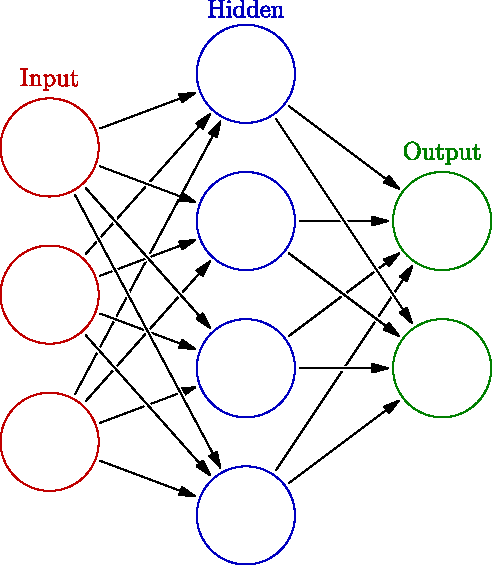
\includegraphics[width=\linewidth]{./fig/3-layer.pdf}
 % 3-layer.pdf: 236x271 pixel, 72dpi, 8.33x9.56 cm, bb=0 0 236 271
 \caption{Glosser.ca / CC-BY-SA-3.0}
\end{figure}
\end{column}

\end{columns}
\end{frame}




\begin{frame}
\frametitle{Why use artificial neural networks for modelling?}
\framesubtitle{Some aspects of their behaviour are like their namesake!}
\begin{itemize}
\item Learn pretty much any input-output data \\ \
 \item Uncover rules on their own about data  \\ \
\item Generalise from what they have learnt \\ \
\item Cope with noise and damage \\ \
\end{itemize}
\end{frame}


\begin{frame}
\frametitle{How does an artificial neural network run?}
\framesubtitle{By using maths, predictably!}
  \begin{columns}[T]
    \begin{column}{.5\textwidth}
    \begin{enumerate}
%      \begin{block}{Run network}
\vfill
\item<1->{Input units are set to a \emph{pattern}} \\ \ \\
\item<3->{Calculate hidden units' states}\only<5-9>{: \\ \ \\
\begin{tabular}{r S[tabformat=3.2] r}% syntax for siunitx v2; for v1 use "tabformat"
$1 \times 0.5~ =$ & $0.5$ &\\
\only<6->{ $1 \times 0.0 ~=$ & $0.0$ &\\}
 \only<7>{$0 \times 0.8 ~=$ & $0.0$ & \\}
  \only<8->{$0 \times 0.8 ~=$ & $0.0$ & +\\
\hline
 & $0.5$ &}
\end{tabular}


}

\ \\ 
\item<11->{Same for output units}\only<13-18>{: \\
\ \\
\begin{tabular}{r S[tabformat=3.2] r}% syntax for siunitx v2; for v1 use "tabformat"
 \only<13-18>{$0.5 \times 0.25~ =$ & $0.125$ &\\}
\only<14-18>{ $0.3 \times 1.5  ~=$ & $0.45$ &\\}
\only<15-18>{ $1.6 \times -0.3 ~=$ & $-0.48$ &\\}
 \only<16-18>{$-0.4 \times 1.1 ~=$ & $-0.44$ &  \\}
 \only<17-18>{$-0.4 \times 1.1 ~=$ & $-0.44$ & + \\
 \hline
 & $-0.345$ & }
\end{tabular}}
\end{enumerate}
% \end{block}
    \end{column}
    \begin{column}{.5\textwidth}
%     \begin{block}{}
% Your image included here
% \begin{figure}
\includegraphics<1>[width=\linewidth]{./fig/3-layer.pdf}
\includegraphics<2-3>[width=\linewidth]{./fig/3-layer_propagate_1.pdf}
\includegraphics<4-8>[width=\linewidth]{./fig/3-layer_propagate_2.pdf}
\includegraphics<9>[width=\linewidth]{./fig/3-layer_propagate_3.pdf}
\includegraphics<10-11>[width=\linewidth]{./fig/3-layer_propagate_4.pdf}
\includegraphics<12-17>[width=\linewidth]{./fig/3-layer_propagate_5.pdf}
\includegraphics<18-19>[width=\linewidth]{./fig/3-layer_propagate_6.pdf}
% \includegraphics<11->[width=\linewidth]{./fig/3-layer_propagate_5.pdf}
%  \only<6>{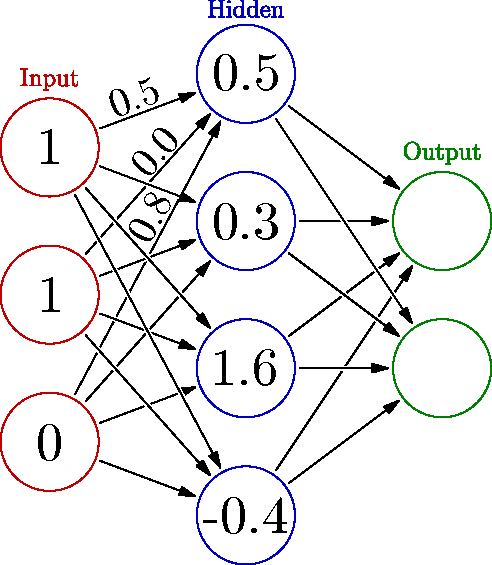
\includegraphics[width=\linewidth]{./fig/3-layer_propagate_4.pdf}}
%   \caption{Glosser.ca / CC-BY-SA-3.0}
% \end{figure}
%     \end{block}
    \end{column}
  \end{columns}
\end{frame}




\begin{frame}
\frametitle{How does an artificial neural network run?}
\framesubtitle{By using maths, predictably!}
  \begin{columns}[T]
    \begin{column}{.5\textwidth}
     \ \\
     \ \\
     
But we/programmers are lazy:
\begin{equation*}
a_i = f \left( \sum_1^N x_j \times w_{ji} \right)
\end{equation*}
where $a_i$ is the unit whose state we want to calculate, $N$ are the units on the previous layer, $w_{ji}$ is the weight on the connection between $i$ and $j$, and $f$ is a function that we will discuss later.

% Which means, to calculate, e.g., $a_1$ multiply all the states in layer before with the incoming weight and then add them up. So in our case all the $x_1~...~x_3$ because $N = 3$.  
% \end{block}
    \end{column}
    \begin{column}{.5\textwidth}
%     \begin{block}{}
% Your image included here
% 	\begin{figure}


	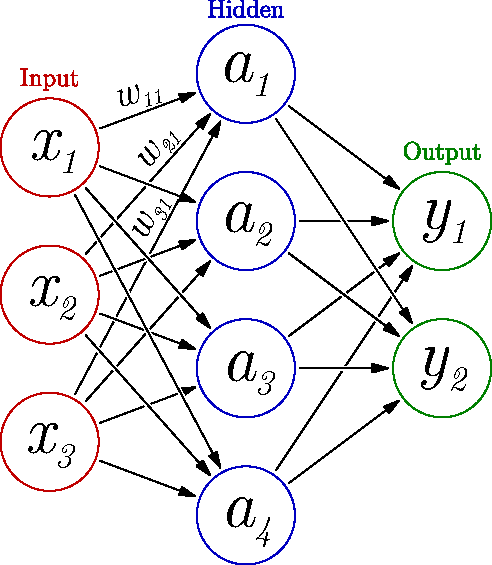
\includegraphics[width=\linewidth]{./fig/3-layer_maths.pdf}
% 	  \caption{Glosser.ca / CC-BY-SA-3.0}
% 	\end{figure}
%     \end{block}
    \end{column}
  \end{columns}
\end{frame}

\begin{frame}
\frametitle{How do networks learn?}
\framesubtitle{Cunning!}
\begin{itemize}
\item Many options: Hebbian learning, back-propagation of error, Boltzmann machine learning, self-organising map algorithm, etc. \\ \

\item All learning algorithms work by changing the connection weights \\ \

\item Learning can be divided into \emph{supervised}, \emph{unsupervised}, and \emph{reinforcement} \\ \ \end{itemize}
\end{frame}

\begin{frame}
\frametitle{Hebbian learning}
\framesubtitle{``Cells that fire together, wire together'' --- Carla Shatz }
  \begin{columns}[T]
    \begin{column}{.5\textwidth}
    \ \\ 
    \onslide<3>{Hebb's rule is very simple but \emph{very unstable}!}
    \onslide<1->{
      \ \\
%     Units that are \emph{on} together in the pattern set are made to \emph{be} on together when the network is run:
      \begin{equation*}
      \Delta w_{ij} = \eta \sum^N_i  x_i \times a_j
      \end{equation*}
      
      \ \\
      
      which means each weight, $w_{ij}$ is changed by a small in/decrement
      }
       \onslide<2-> {      \ \\ 

      If $x_i$ or $a_j$ is on, then the other will also be on}

    \end{column}
    \begin{column}{.5\textwidth}
%     \begin{block}{}
% Your image included here
\begin{figure}
 
 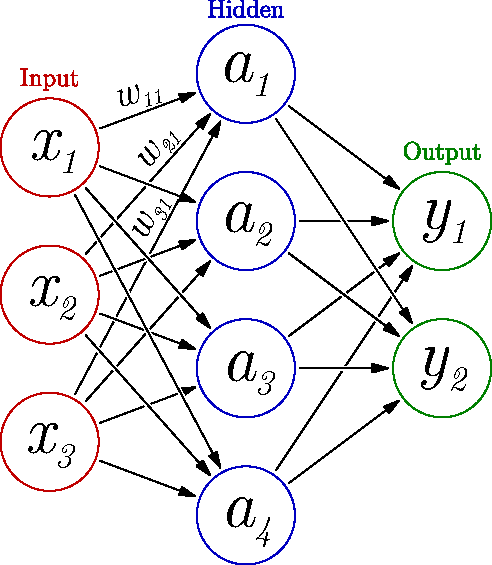
\includegraphics[width=\linewidth]{./fig/3-layer_maths.pdf}
%   \caption{Glosser.ca / CC-BY-SA-3.0}
\end{figure}
%     \end{block}
    \end{column}
  \end{columns}
\end{frame}




\begin{frame}
\frametitle{The perceptron}
\framesubtitle{A simple classifier}
  \begin{columns}[T]
    \begin{column}{.5\textwidth}    \ \\ \ \\ 
    \ \\
    \begin{itemize}
    
 
     \item Created in 1957 at the Cornell Aeronautical Laboratory by Frank Rosenblatt  \\ \
\item Linear classifier \\ \

\item Simplest form of feedforward network \\ \

% \item Consists of two layers of units \\ \
% \item No hidden units \\ \
\end{itemize}

    \end{column}
    \begin{column}{.5\textwidth}
%     \begin{block}{}
% Your image included here
\begin{figure}
 
 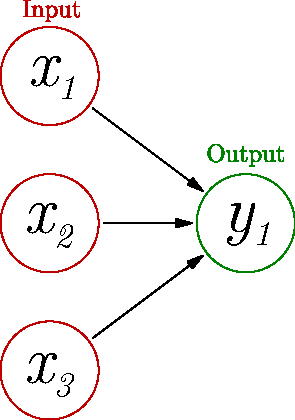
\includegraphics[width=0.9\linewidth]{./fig/perceptron.pdf}
%   \caption{Glosser.ca / CC-BY-SA-3.0}
\end{figure}
%     \end{block}
    \end{column}
  \end{columns}
\end{frame}


\begin{frame}
\frametitle{How does the perceptron learn?}
\framesubtitle{Maths again!}
  \begin{columns}[T]
    \begin{column}{.5\textwidth} 
    \ \\
    \ \\
\begin{enumerate}

 \item<1-> Initialise weights
 \\ \
 \item<2-> Run network \onslide<2>{using: 
 
 \begin{equation*}
y_j = f \left( \sum_1^N w_i \times x_i \right)
 \end{equation*} 
 \\ \
 
same as always!
\\ \
}

% \item<3-> Update weights using: 
%  
%  \begin{equation*}
%   \Delta w_i = \eta ( d_j - y_j ) \times x_{i}
%  \end{equation*} 
%   \ \\
%  
%  where $d$ is what we want $y$ to be given $x_i$, and $\eta$ is the learning rate.

 \end{enumerate}

    \end{column}
    \begin{column}{.5\textwidth}
%     \begin{block}{}
% Your image included here
\begin{figure}
 
 \includegraphics<1->[width=0.9\linewidth]{./fig/perceptron_maths.pdf}
%   \caption{Glosser.ca / CC-BY-SA-3.0}
\end{figure}
%     \end{block}
    \end{column}
  \end{columns}
\end{frame}


\begin{frame}
\frametitle{How does the perceptron learn?}
\framesubtitle{Maths again!}
  \begin{columns}[T]
    \begin{column}{.5\textwidth} 
        \  \\
 \   \\ 
\begin{enumerate}
 \item Initialise weights
 
 \ \\
 \item Run network
 
 \ \\
 
 \item Update weights using:

\end{enumerate}
 
 \begin{equation*}
  \Delta w_i = \eta ( d_j - y_j ) \times x_{i}
 \end{equation*} 
  \ \\
 
 where $d$ is what we want $y$ to be given $x_i$, and $\eta$ is the learning rate.

    \end{column}
    \begin{column}{.5\textwidth}
%     \begin{block}{}
% Your image included here
\begin{figure}
 
 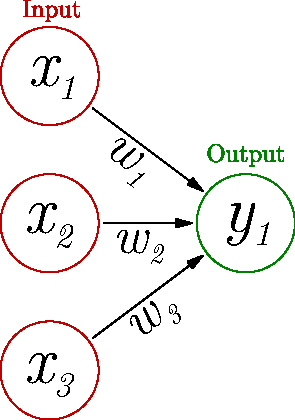
\includegraphics[width=0.9\linewidth]{./fig/perceptron_maths.pdf}
%   \caption{Glosser.ca / CC-BY-SA-3.0}
\end{figure}
%     \end{block}
    \end{column}
  \end{columns}
\end{frame}


\begin{frame}
\frametitle{How does the perceptron learn?}
\framesubtitle{Maths again!}
  \begin{columns}[T]
    \begin{column}{.5\textwidth} 
        \  \\
 \   \\ 
\begin{enumerate}
 \item<1-> Initialise weights
 
 \ \\
 \item<1-> Run network
 
 \ \\
 
 \item<1-> Update weights
 
  \ \\
 
 \item<1-> Repeat 2 and 3
 
 \ \\

 \item<2> When do we stop?
\end{enumerate}


    \end{column}
    \begin{column}{.5\textwidth}
%     \begin{block}{}
% Your image included here
\begin{figure}
 
 \includegraphics<1->[width=0.9\linewidth]{./fig/perceptron_maths.pdf}
%   \caption{Glosser.ca / CC-BY-SA-3.0}
\end{figure}
%     \end{block}
    \end{column}
  \end{columns}
\end{frame}




\begin{frame}
\frametitle{The end}
\framesubtitle{}
        \  \\
 \   \\ 

 \Huge Time to program a perceptron!
\end{frame}




\end{document}
